\chapter{System Models}

\section{Scenarios}
The scenarios are based on Node.js based web applications on a server running ROOT and rootJS\\
Bindings do not extend the basic functionality of the underlying framework.\\
We therefore only assume a fictional application, using our API, to be the user of rootJS.\\


Scenario 1: //TODO fix layout and create UML\\
WebViewer, a browser based GUI for realtime representation of root graphs
	rootJS is up and running initialize has already been executed
	WebViewer calls the API method to get graphical output of the data ROOT has currently loaded
	\indent rootJS processes the request and calls the corresponding ROOT functionality
	\indent rootJS receives ROOT output and streams it to the Webviewer client
webViewer uses the provided data to display the graph on its GUI

\indent	Node.js invokes ROOT I/O operations\\
\indent \indent		ROOT loads data and provides raw visualization data\\
\indent	Node.js serializes data and streams it to the web viewer\\
Web viewer receives data and renders it in the browser\\

\section{Use Cases}
Our bindings do not add to the core functionality of ROOT. Therefore 
we decided to give some examples on how the bindings might be used. The 
user in this case is a nodeJS based application, that uses our bindings 
to interact with root. Because the actual implementation is not yet 
decided upon, our use cases contain only samples of simple interaction 
between such an app and root.
\begin{figure}[htb]
	\centering
	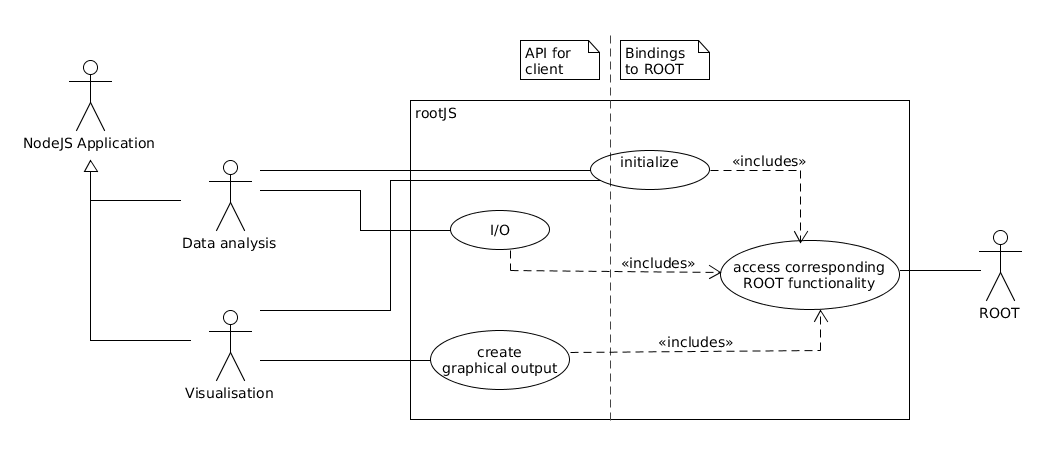
\includegraphics[width=18cm]{./latex/resources/usecaseOverview.png}
	\caption{use case overview}
\end{figure}

\pagebreak[4]

\section{Object Models}
Figure 6.2 illustrates what the rootJS architecture may look like.
Client applications relying on this architecture will incorporate with the ROOT framework through a \textit{ROOTPrototype} object.
The API's entry point method \textit{ROOTPrototype::init} uses V8 to create the actual interface to the available variables, functions and classes of ROOT.\\
Functions provided through this interface internally call \textit{methodProxy} to determine the associated ROOT function via the callee's function name. This allows handling of supplied callback functions by passing them over the \textit{args} parameter.\\
Constructor functions provided through the interface internally call \textit{classProxy} instead of \textit{methodProxy} to generate encapsulating JavaScript objects through the \textit{ProxyObjectFactory}.
A \textit{ROOTPrototype} object provides the \textit{globalGetter} and \textit{globalSetter} methods to access ROOT's global variables. Again interfacing with global objects is done through \textit{ProxyObject}s generated by the \textit{ProxyObjectFactory}.
\\ \\
The \textit{ProxyObjectFactory} instantiates a class realizing the \textit{ProxyObject} interface. The actual class type is given through the supplied \textit{type} parameter.
If the \textit{getV8Handle} method is called on \textit{ProxyObject}s encapsulating C++ scalar types (like int, long, string, etc.) it will simply return the corresponding \textit{v8::Handle} with the value at a defined address in memory.\\
However, calling the \textit{getV8Handle} method on \textit{ProxyObject}s encapsulating C++ objects will prompt recursive calls to the \textit{ProxyObjectFactory} for every (member) variable the native object holds. This allows to dynamically assemble the encapsulating object.
To handle cyclic references a caching mechanism (\textit{ProxyObjectCache}), that stores already created \textit{v8::Handle}s, is used.\\
A sample process of interfacing with a ROOT object using this architecture is shown in Figure 6.4.

\begin{figure}[htb]
	\centering
	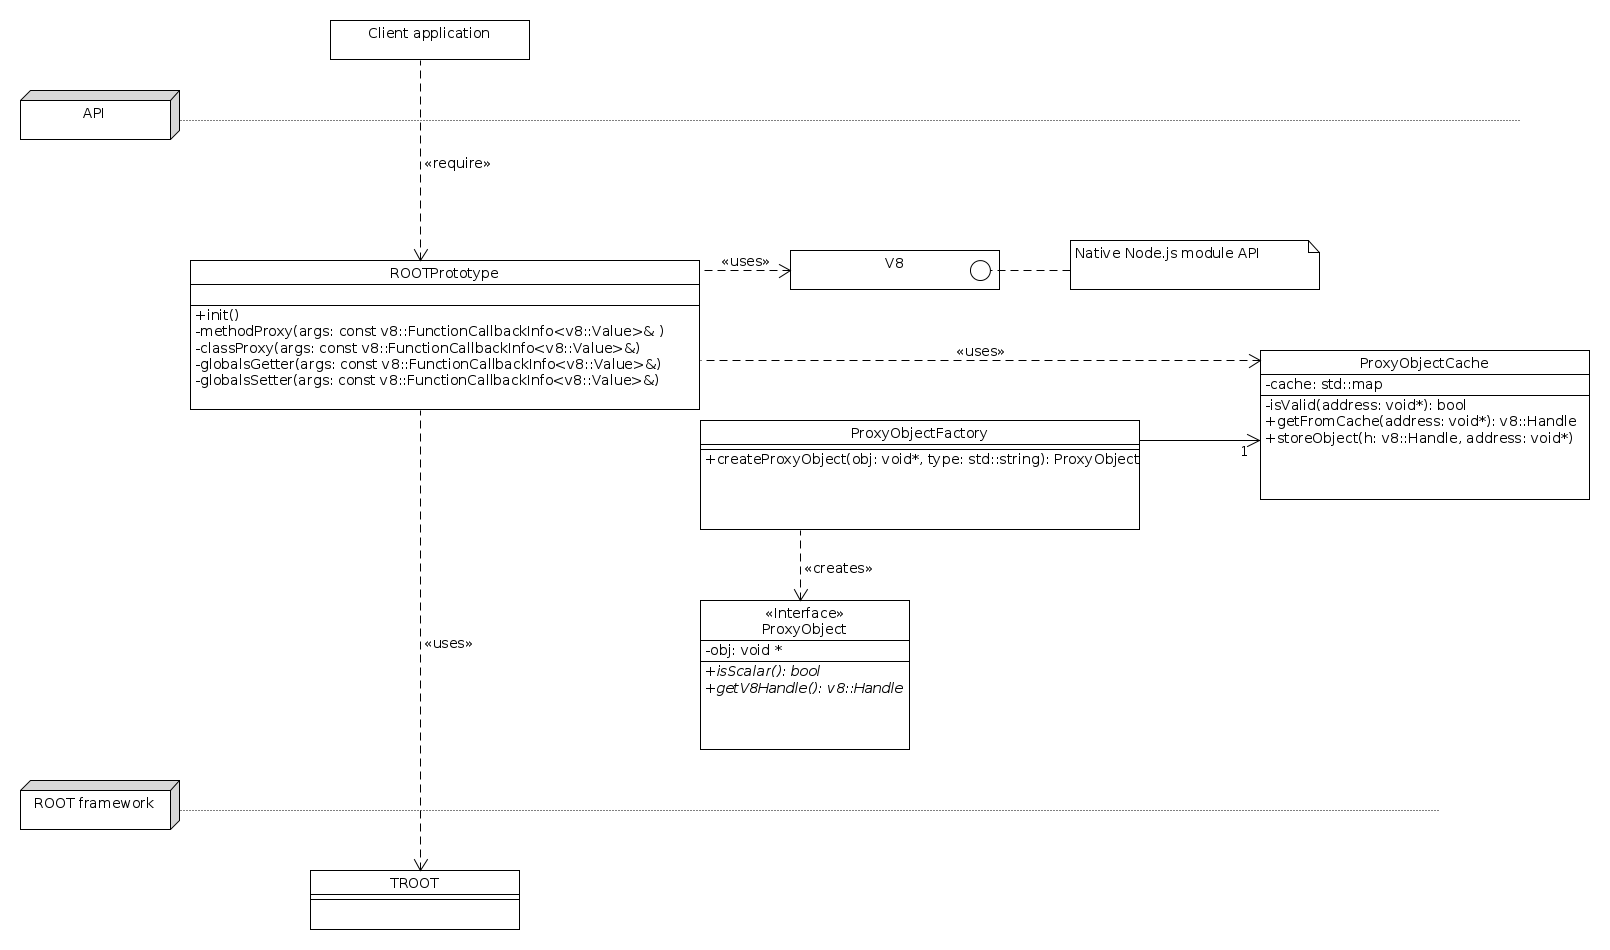
\includegraphics[width=18cm]{./latex/resources/architecture.png}
	\caption{basic architecture draft}
\end{figure}

\pagebreak[4]

\section{Dynamic Models}
The following figure shows how rootJS initializes upon being called the first time by a client application. As bindings do not add any functionality of their own, the client application is not further specified. After the bindings are initialized the client application may use any ROOT functionality through a \textit{ROOTPrototype} object provided by the rootJS API.

\begin{figure}[htb]
	\centering
	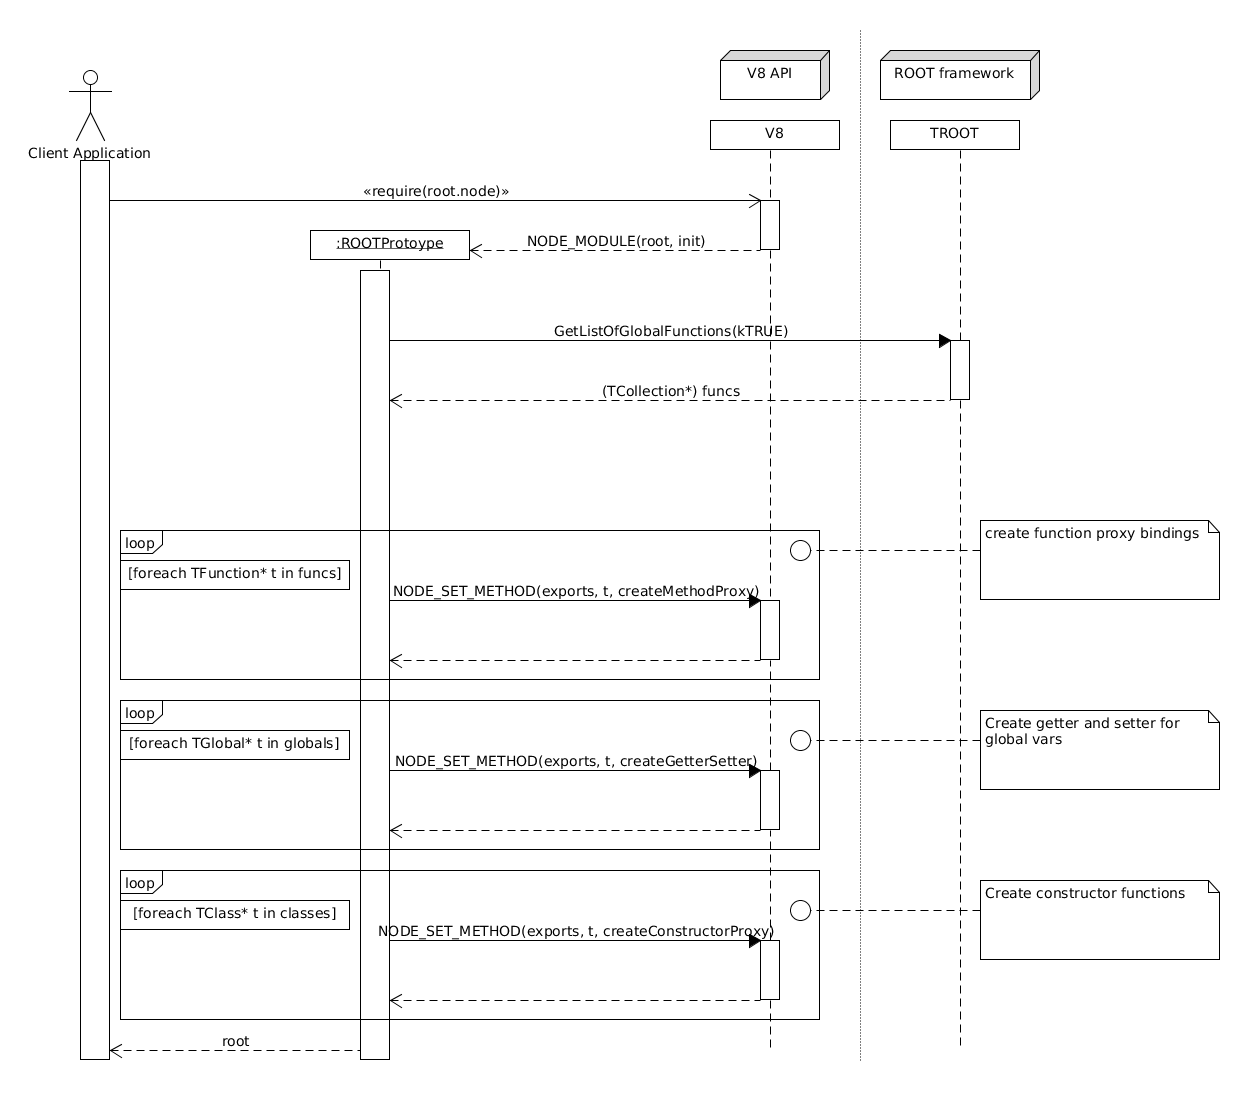
\includegraphics[width=18cm]{./latex/resources/startupSequence.png}
	\caption{basic startup sequence}
\end{figure}

The following figure shoes how to open a root file via rootJS, after the usual initialization process has been completet (see above) a TFile object is beeing created using the rootJS API. A callback is provided because the file is beeing parsed by ROOT during the opening process, which might take some time depending on file size and complexity. The rootJS bindings call the TFile constructor before returning to the JavaScript application via callback, the constructor is beeing called by the class proxy. After the construction phase rootJS has a valid TFile object, which is then handed over to the CreateProxyObject factory method which creates the correct proxy object. The factory object recursively creates a v8 handle which is returned to the JavaScript code running in node, in this case via callback.
\begin{figure}[htb]
	\centering
	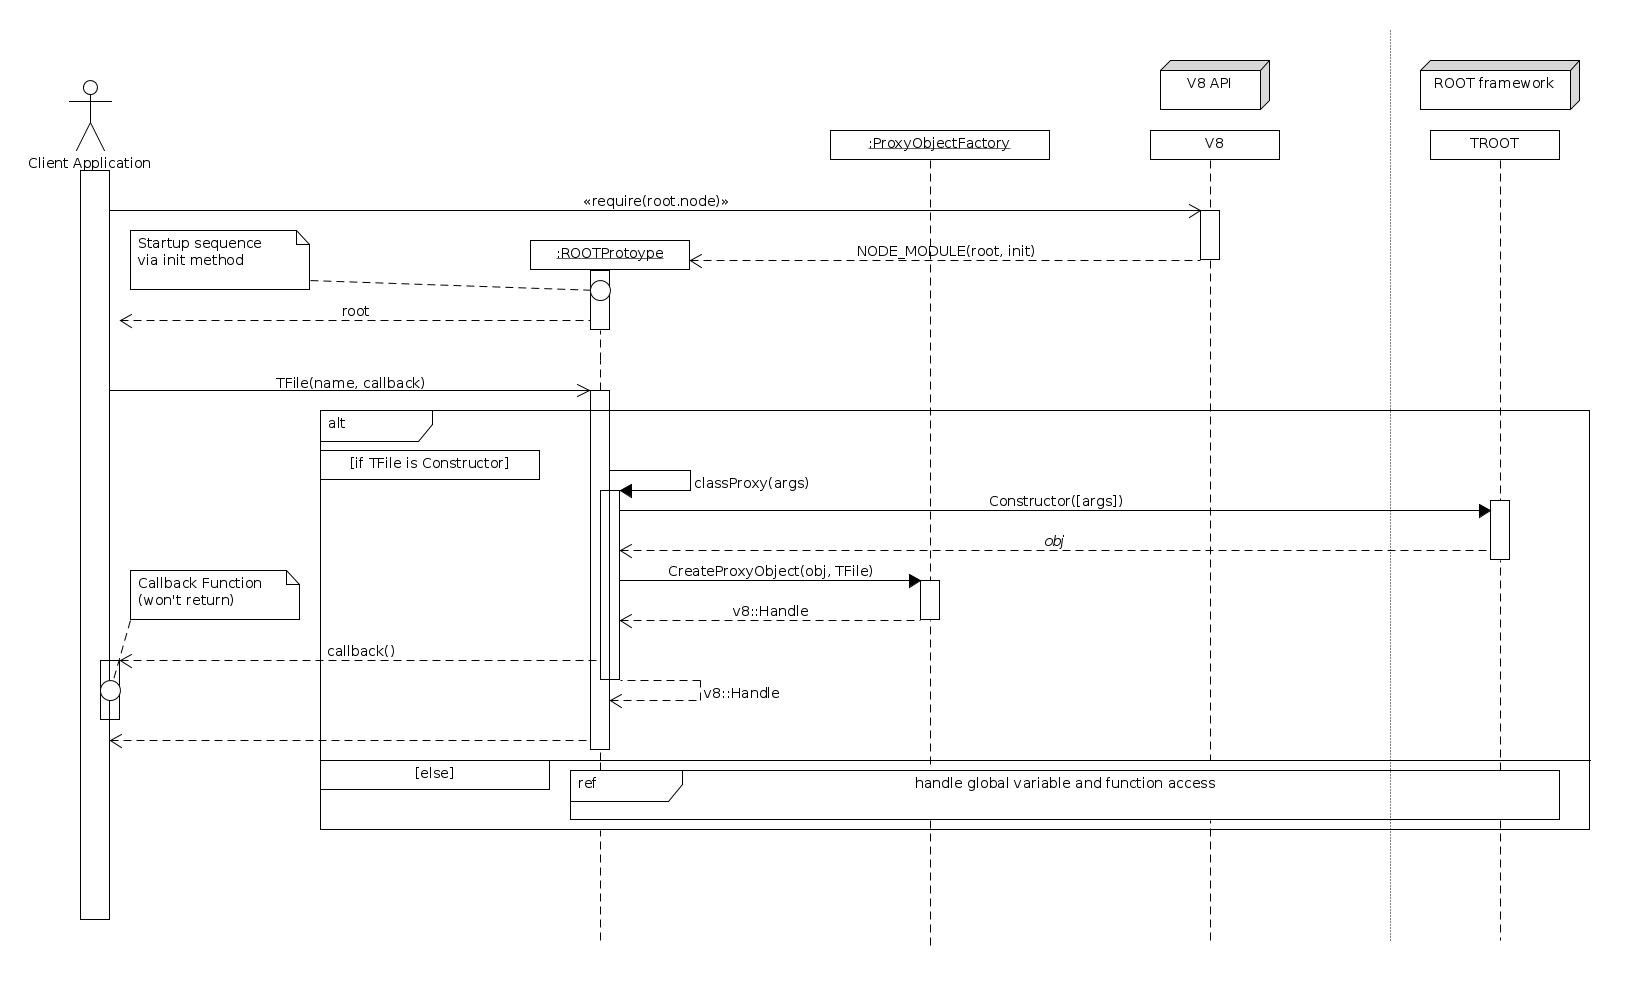
\includegraphics[width=18cm]{./latex/resources/fileOpen.png}
	\caption{basic sequence used for opening a file}
\end{figure}
